\chapter{Конструкторский раздел}

\section{Диаграмма состояний (IDEF0)}
На рисунках \ref{fig:idef01} и \ref{fig:idef02} показаны соответственно нулевой и первый уровни диаграммы IDEF0, отображающие процесс мониторинга информации о процессах.

\begin{figure}[H]
	\centering
	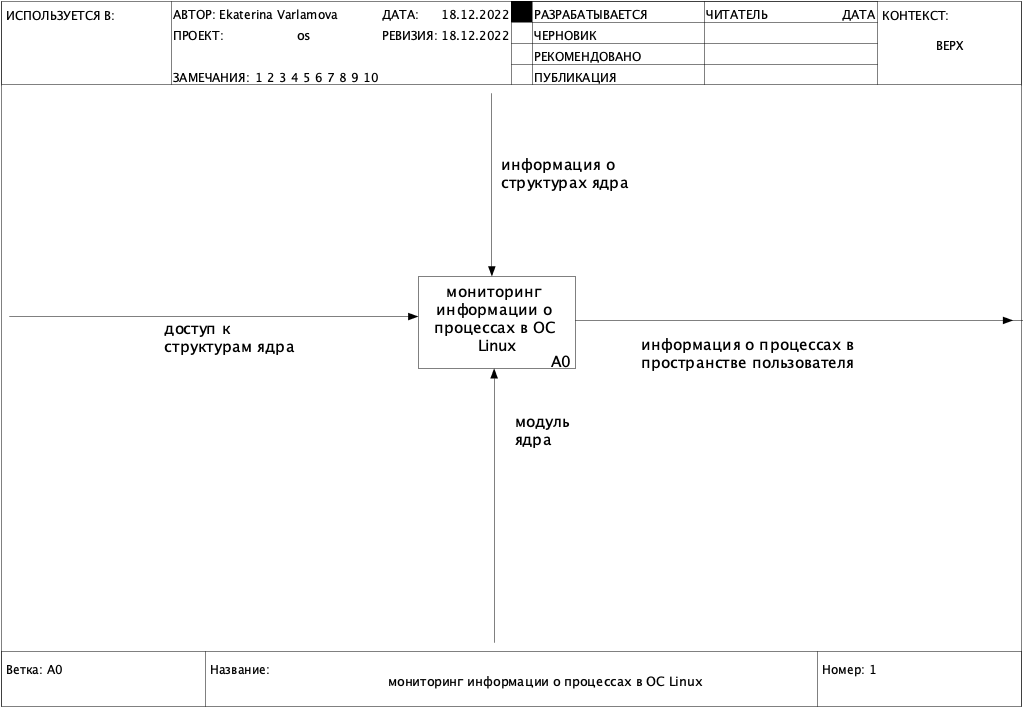
\includegraphics[scale=0.32]{img/01_A0.png}
	\caption{IDEF0 нулевого уровня.}
	\label{fig:idef01}
\end{figure}

\begin{figure}[H]
	\centering
	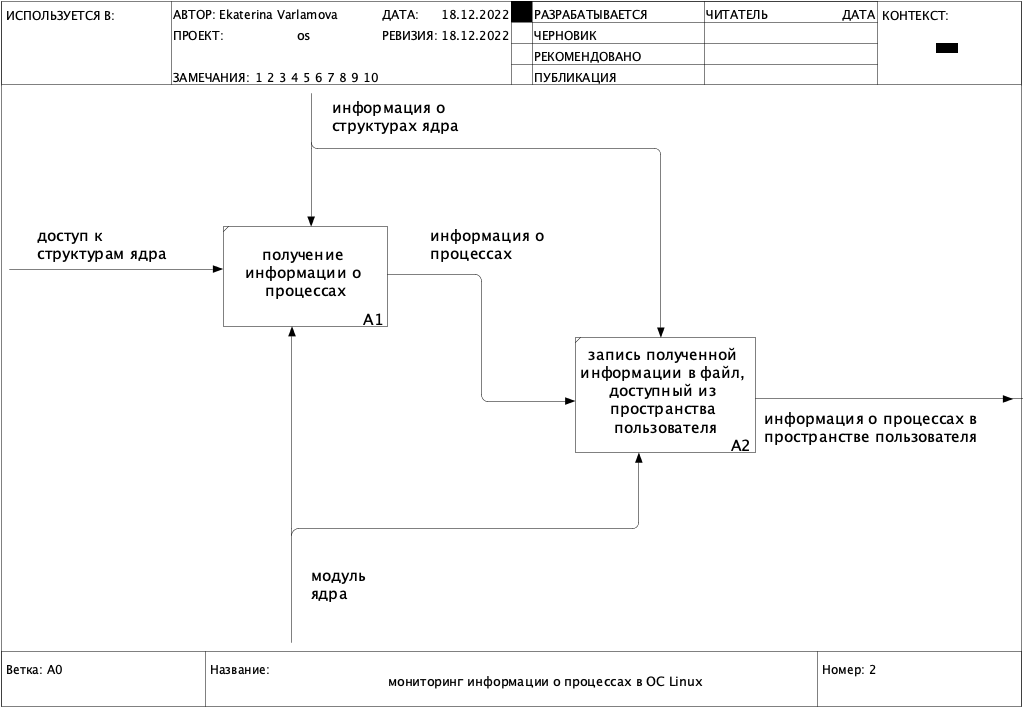
\includegraphics[scale=0.32]{img/02_A0.png}
	\caption{IDEF0 первого уровня.}
	\label{fig:idef02}
\end{figure}
\newpage
\section{Алгоритмы для мониторинга информации о процессах}

\textbf{Алгоритмы модуля ядра}

На рисунке \ref{fig:read} представлен алгоритм вывода информации о процессах в файл в /proc. Данный алгоритм должен быть выполнен в момент чтения файла /proc. В алгоритме также предполагается, что файл в /proc уже создан. 

\begin{figure}[H]
	\centering
	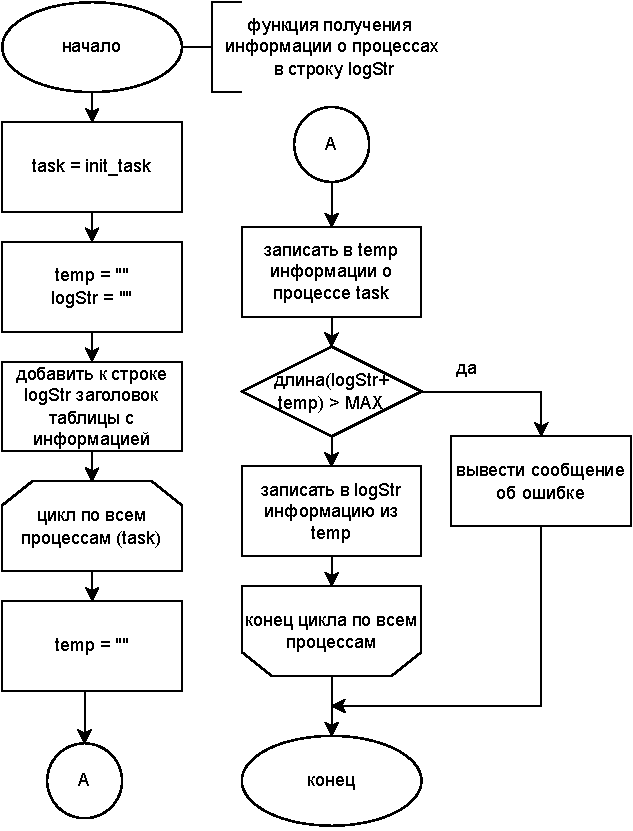
\includegraphics[scale=1]{img/os-l1.pdf}
	\caption{Алгоритм вывода информации о процессах в файл в /proc }
	\label{fig:printTasks}
\end{figure}
\newpage
На рисунке \ref{fig:read} представлен алгоритм получения информации о процессах из структур ядра. 

\begin{figure}[H]
	\centering
	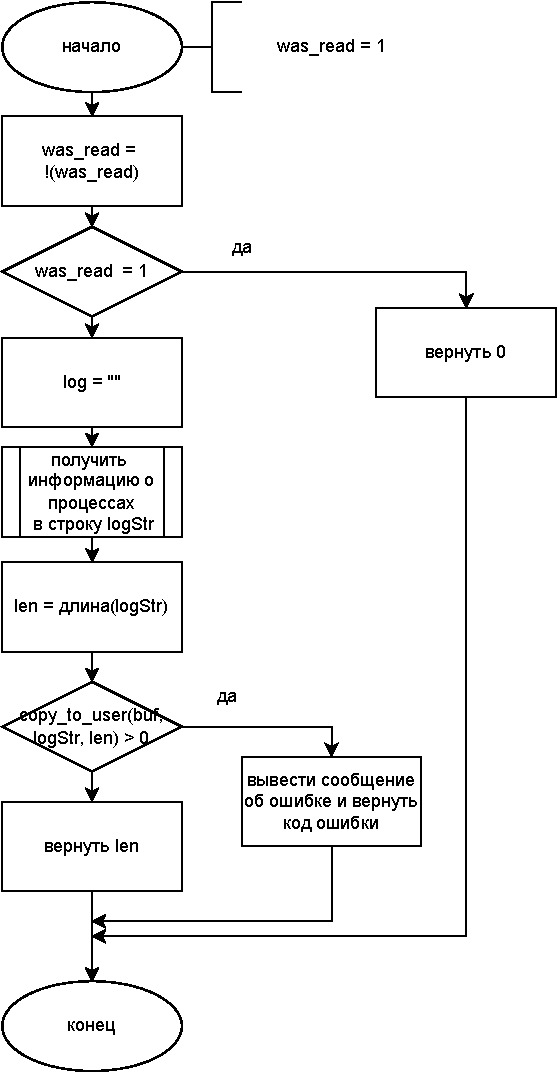
\includegraphics[scale=1]{img/os-l2.pdf}
	\caption{Алгоритм получения информации о процессах из структур ядра}
	\label{fig:read}
\end{figure}

\textbf{Алгоритм получения информации из файла в procfs в пространстве пользователя}

Для исследования процессов в динамике был разработан алгоритм получения информации из /proc в течение заданного количества секунд с интервалом в одну секунду. Алгоритм представлен на рисунке \ref{img:osprogram.pdf}

\begin{figure}[H]
	\centering
	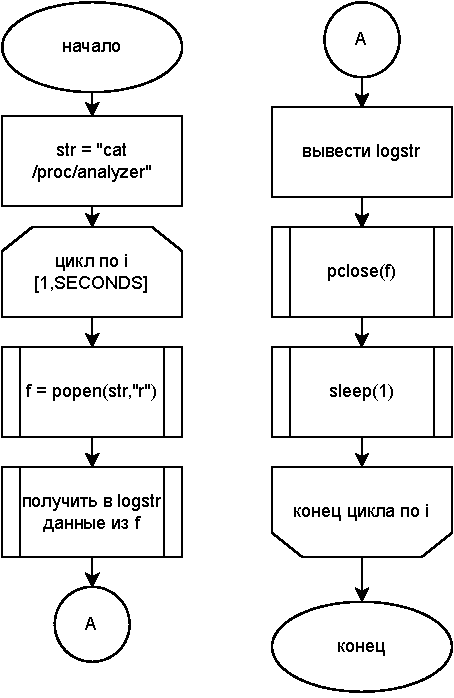
\includegraphics[scale=1]{img/os-program.pdf}
	\caption{Алгоритм получения информации из /proc}
	\label{img:osprogram.pdf}
\end{figure}

\section{Структура разработанного ПО}
На рисунке \ref{fig:structure} представлена структура разработанного ПО. 
\begin{figure}[H]
	\centering
	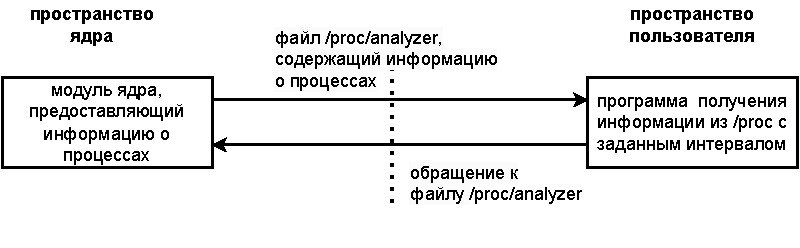
\includegraphics[scale=1]{img/os-structure.pdf}
	\caption{Структура ПО}
	\label{fig:structure}
\end{figure}
